

\tikzset{every picture/.style={line width=0.75pt}} %set default line width to 0.75pt        

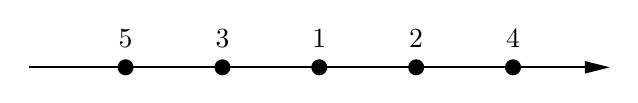
\begin{tikzpicture}[x=0.75pt,y=0.75pt,yscale=-1,xscale=1]
%uncomment if require: \path (0,300); %set diagram left start at 0, and has height of 300

%Straight Lines [id:da7449686192404181] 
\draw    (100,153) -- (146.67,153) ;
\draw [shift={(146.67,153)}, rotate = 0] [color={rgb, 255:red, 0; green, 0; blue, 0 }  ][fill={rgb, 255:red, 0; green, 0; blue, 0 }  ][line width=0.75]      (0, 0) circle [x radius= 3.35, y radius= 3.35]   ;
%Straight Lines [id:da9017019116760947] 
\draw    (146.67,153) -- (193.33,153) ;
\draw [shift={(193.33,153)}, rotate = 0] [color={rgb, 255:red, 0; green, 0; blue, 0 }  ][fill={rgb, 255:red, 0; green, 0; blue, 0 }  ][line width=0.75]      (0, 0) circle [x radius= 3.35, y radius= 3.35]   ;
%Straight Lines [id:da26753414986637103] 
\draw    (193.33,153) -- (240,153) ;
\draw [shift={(240,153)}, rotate = 0] [color={rgb, 255:red, 0; green, 0; blue, 0 }  ][fill={rgb, 255:red, 0; green, 0; blue, 0 }  ][line width=0.75]      (0, 0) circle [x radius= 3.35, y radius= 3.35]   ;
%Straight Lines [id:da9354128008118774] 
\draw    (240,153) -- (286.67,153) ;
\draw [shift={(286.67,153)}, rotate = 0] [color={rgb, 255:red, 0; green, 0; blue, 0 }  ][fill={rgb, 255:red, 0; green, 0; blue, 0 }  ][line width=0.75]      (0, 0) circle [x radius= 3.35, y radius= 3.35]   ;
%Straight Lines [id:da7011463755992022] 
\draw    (286.67,153) -- (333.33,153) ;
\draw [shift={(333.33,153)}, rotate = 0] [color={rgb, 255:red, 0; green, 0; blue, 0 }  ][fill={rgb, 255:red, 0; green, 0; blue, 0 }  ][line width=0.75]      (0, 0) circle [x radius= 3.35, y radius= 3.35]   ;
%Straight Lines [id:da5013137889897423] 
\draw    (333.33,153) -- (378,153) ;
\draw [shift={(380,153)}, rotate = 180] [fill={rgb, 255:red, 0; green, 0; blue, 0 }  ][line width=0.08]  [draw opacity=0] (12,-3) -- (0,0) -- (12,3) -- cycle    ;

% Text Node
\draw (240,145) node [anchor=south] [inner sep=0.75pt]   [align=left] {1};
% Text Node
\draw (286.67,145) node [anchor=south] [inner sep=0.75pt]   [align=left] {2};
% Text Node
\draw (193.33,145) node [anchor=south] [inner sep=0.75pt]   [align=left] {3};
% Text Node
\draw (333.33,145) node [anchor=south] [inner sep=0.75pt]   [align=left] {4};
% Text Node
\draw (146.67,145) node [anchor=south] [inner sep=0.75pt]   [align=left] {5};


\end{tikzpicture}
